\documentclass[10pt,aps,pre,preprint,superscriptaddress]{revtex4-1}

\usepackage{amsmath,amsthm}
\usepackage{amssymb}
\usepackage{amscd}
\usepackage{wasysym}
\usepackage[ansinew]{inputenc}
\usepackage[T1]{fontenc}
\usepackage{ae,aecompl}
\usepackage{hyperref}

   
    \usepackage[pdftex]{graphicx}
%    \DeclareGraphicsExtensions{.pdf}

\usepackage{color}
\definecolor{red}{rgb}{1,0,0}
\definecolor{blue}{rgb}{0,0,1}
\definecolor{green}{rgb}{0,0.5,0}
\definecolor{magenta}{rgb}{1,0,1}

\newcommand{\marc}[1]{\textcolor{red}{#1}}
\newcommand{\dirk}[1]{\textcolor{blue}{#1}}
\newcommand{\debsankha}[1]{\textcolor{magenta}{#1}}
\newcommand{\ceil}[1]{\left\lceil#1\right\rceil}


% -- new commands -------------------------------------------

\newtheorem{thm}{Theorem}
\newtheorem{defn}[thm]{Definition}

\newcommand{\abs}[1]{\vert#1\vert}
\newcommand{\be}{\begin{equation}}
\newcommand{\ee}{\end{equation}}
\newcommand{\bea}{\begin{eqnarray}}
\newcommand{\eea}{\end{eqnarray}}
\newcommand{\nn}{\nonumber}
\newcommand{\ket}[1]{|#1\rangle}
\newcommand{\bra}[1]{\left\langle#1\right|}
\newcommand{\braket}[2]{\langle{#1}|{#2}\rangle}
\newcommand{\eye}{\mbox{$\mbox{1}\!\mbox{l}\;$}}
\newcommand{\E}{{\cal E}}
\newcommand{\N}{{\cal N}}
\newcommand{\EE}{\mathbf{E}}
\newcommand{\PP}{\mathbf{P}}
\newcommand{\HH}{\mathcal{H}}
\newcommand{\tr}{{\rm tr}}
\renewcommand{\vec}[1]{\boldsymbol{#1}}
\newcommand{\R}{\mathcal{R}}
\newcommand{\F}{\mathcal{F}}
\newcommand{\PR}{\mathcal{PR}}
\newcommand{\floor}[1]{\left\lfloor #1 \right \rfloor}
\newcommand{\maxp}{S(\vec{P})}
\newcommand{\maxf}{R(\vec{P})}

\newtheorem{lemma}{Lemma}
\newtheorem{theorem}{Theorem}
\newtheorem{corr}{Corollary}
\newtheorem{claim}{Claim}
\newtheorem{problem}{Problem}
\newtheorem{obs}{Observation}
\newtheorem{defi}{Definition}

% --- front matter ---------------------------------------------

\begin{document}
\bibliographystyle{apsrev}
\title{Geometric frustration and multistability in oscillator networks}

\author{Dirk Witthaut}
\affiliation{Network Dynamics, Max Planck Institute for Dynamics and Self-Organization (MPIDS), Am Fassberg 17, D--37077 G\"ottingen, Germany}

\author{Debsankha Manik}
\affiliation{Network Dynamics, Max Planck Institute for Dynamics and Self-Organization (MPIDS), Am Fassberg 17, D--37077 G\"ottingen, Germany}

\author{Who else}
\affiliation{Network Dynamics, Max Planck Institute for Dynamics and Self-Organization (MPIDS), Am Fassberg 17, D--37077 G\"ottingen, Germany}


\author{Marc Timme}
\affiliation{Network Dynamics, Max Planck Institute for Dynamics and Self-Organization (MPIDS), Am Fassberg 17, D--37077 G\"ottingen, Germany}
\affiliation{Faculty of Physics, Georg August University G\"ottingen,
  Germany}



\date{\today }


\begin{abstract}
We introduce the concept of geometric frustration for networks
of coupled oscillators. This concept readily explains some 
surprising features of the steady states of the network 
including Braess' paradox.
Using this approach  
we show that multistability is generally possible and derive
upper bounds for the number of stable steady states depending
on the network topology.
\end{abstract}


\maketitle

% --- Content --------------------------------------------------------------------

\section{Introduction}

\dirk{XXX FIXME XXX}


\section{From Kuramoto oscillators to power grids}

Coupled oscillator models are ubiquitous in science and technology,
describing the collective dynamics of various systems form
the micro- to the macroscale. Research on coupled
oscillators dates back to Christian Huygens, who noticed that
two clocks synchronize when they are coupled \cite{Huyg93}.
One of the most important mathematical models was introduced
by Kuramoto \cite{Kura75,Kura84} and successfully applied
to describe the collective dynamics 
of coupled Josephson junctions \cite{Wies96}
neuronal networks \cite{Vare01}
chemical oscillators \cite{Kiss02}
and a variety of other synchronization phenomena
\cite{Stro00,Aceb05,Aren08},

The model describes the dynamics of $N$ coupled limit cycle 
oscillators \cite{Kura84}. The equations of motions for the 
phases $\phi_j, \; j = 1,\ldots,N$ is given by
\be
   \frac{d}{dt} \phi_j = \omega_j  + \sum_{\ell = 1}^N
      K _{j,\ell} \sin(\phi_\ell - \phi_j).
   \label{eqn:kuramoto}
\ee 
The coupling matrix is assumed to be symmetric, $K _{j,\ell} = K _{\ell,j}$.
It is useful to describe the system as a graph $G(V,E)$, whose vertex set $V$ 
is identical with the set of oscillator, and edge set $E$ is the set of all inter-oscillator 
couplings, i.e., all pairs with $K _{\ell,j} > 0$.


A similar model of second-order oscillators describes the collective phenomena of 
animal flocks \cite{Erme91,Ha10} or human crowds \cite{Stro05} as well as the 
coarse-scale dynamics of power grids \cite{Berg81,Fila08,12powergrid,Mott13,Dorf13}.
In this model one considers $N$ coupled synchronous machines, generators or motors, 
whose state is completely described by their phase $\phi_j$ and the phase 
velocity $\dot \phi_j$ relative to the reference frame of the grid, which is rotating
at 50 Hz or 60 Hz, respectively.   
The acceleration (deceleration) of the machines is proportional to the mechanical 
power $P_j$ generated (consumed) by the machine including friction losses plus
the electric power exchanged with the grid. The detailed equations of motion a
re derived from the conservation of energy with the result
\be
   \frac{d^2}{dt^2} \phi_j = P_j - \alpha \phi_j
             + \sum_{\ell = 1} K _{j,\ell} \sin(\phi_\ell - \phi_j). 
  \label{eqn:power}
\ee
The couplings constants are given by $K_{j,\ell} = U^2 B_{j,\ell}$ is determined
by the voltage of the grid, which is assumed to be constant, and the admittance
of the electrical transmission line joining node $j$ and node $\ell$.  
In this case the flow of electric real power between the nodes $\ell$ and $j$ is given by 
$F_{j,\ell}= K _{j,\ell} \sin(\phi_\ell - \phi_j) 
=  K _{j,\ell}  \Delta_{j,\ell}$.


Two types of synchronization have to be distinguished in oscillator networks.
Traditionally, the emergence of partial synchrony has received the most
interest in the physics community \cite{Kura75,Kura84,Stro00,Aceb05}.
In his seminal work, Kuramoto investigated a set of oscillators with global coupling,
$K_{j,\ell} = K/N$ and natural frequencies drawn at random from a unimodal symmetric 
distribution $g(\omega)$. If the coupling constant $K$ exceeds a critical value $K_c$, 
a fraction of the oscillators start to synchronize in the sense that they rotate at the 
same angular velocity, although their natural frequencies differ. 
In this state, the phases of parts of the oscillators are ordered, but they are not
strictly phase-locked. In particular, the phase difference of two synchronized
oscillators $|\phi_j - \phi_\ell|$ is generally small, but it is not constant.

In this article, we analyze the properties of \emph{globally phase-locked states},
where all oscillators synchronize and the phase differences $|\phi_j - \phi_\ell|$ 
are constant for all pairs $(j,\ell)$.  These states are especially important in the 
case of power grids, as they describe the regular synchronous operation of the grid
\cite{Berg81,Fila08,12powergrid,Mott13,Dorf13}.
If this state is lost due to local outages or accidents, the grid will fragment into
asynchronous islands which can no no longer exchange electric energy. 
For instance, the European power grid fragmented into three asynchronous 
areas on November 4th 2006 after the shutdown of one transmission line
in Northern Germany. As a result, south-western Europe suffered an undersupply 
on the order of 10 GW and approximately 10 million households were disconnected
\cite{UCTE07}.


Without loss of generality, we can assume that $\sum_j \omega_j = 0$ or 
$\sum_j P_j = 0$, respectively. Otherwise we can simply invoke a transformation
to co-rotating frame of reference.  The globally phase-locked states then correspond 
to the \emph{stationary states} of the system. Both for the Kuramoto model and t
he power grid model, these states are given by the solutions of the equations
\be
       \omega_j  + \sum_{\ell = 1}^N
      K _{j,\ell} \sin(\phi_\ell - \phi_j) =0 \qquad
     \forall j = 1,\ldots, N,
    %\label{eqn:sstate}
    \label{eqn:def-steady-state}
\ee
replacing $\omega_j$ by $P_j$ for the power grid.
In the following we analyze the influence of the network
topology given by the coupling matrix $K_{j,\ell}$ on the
existence of a stationary state. Our results obviously hold
for both models, nevertheless our reasoning heavily relies
on the interpretation of $F_{j,\ell}= K _{j,\ell} \sin(\phi_\ell - \phi_j)$
as a flow which is inspired from the power grid model. 
One can generalize our results to include arbitrary coupling
functions $f$ instead of the sine (see, e.g., \cite{Wata93,Bick11}). 
In the following we mostly restrict ourselves to the common 
sine coupling for the sake of clarity.

\dirk{XXX Dear Debsankha, I think that we should not include a section on the transition
to partial synchrony in the original Kuramoto model. It would be misleading, as we are NOT
interested in this transition but rather in the transition to global phase-locking. XXX}

%\section{Role of network topology in stable operation}
%
%\subsection{Completely coupled infinite dimensional systems}
%\debsankha{I'm writing a summary of significant progress made so far on the 
%topic of phase-locked operation of non-globally coupled Kuramoto oscillators.}
%
%Numerous physical and biological systems are modelled by the Kuramoto model 
%\eqref{eqn:kuramoto}. In 1975, Kuramoto made extensive research in \emph{completely coupled }
%and \emph{infinite dimensional} systems with natural frequencies $\omega$ distributed according to a 
%normalized pdf $g(\omega)$ satisfying $g(\omega)=g(-\omega)$.  He showed that in those systems, a phase transition occurs 
%when the uniform global coupling $K$ is increased gradually. To this end, he 
%defined the \emph{order parameter} $r$
%\begin{equation}
%\label{eq:kuramoto_r}
%re^{i\Psi}=\frac{1}{N}\sum_j e^{i\theta_j}. 
%\end{equation}
%
%At low $K$, the 
%oscillators are uniformly distributed on 
%the unit circle.  However, after a critical coupling, 
%$K>K_c=\frac{2}{\pi g(0)}$, a \emph{partial phase locking happens:} all 
%oscillators with $-Kr<\omega<Kr$ phase lock such that
%\begin{equation}
%Kr\sin{(\theta-\Psi)}=\omega.  
%\end{equation}
%
%As $K$ is increased further, $r$ keeps increasing: and therefore, more 
%oscillators enter the phase locked state from the incoherent state.  If the 
%frequency distribution $g(\omega)$ has a bounded support, there exists a 
%$K_{lock}>K_c$ at which all the oscillators phase lock.  At the 
%$K\gtrapprox K_c$ limit, there exists a scaling law
%\begin{equation}
%\label{eq:kuramoto-scaling}
%r\sim\sqrt{\frac{-16(K-K_c)}{\pi K_c^4g''(0)}}. 
%\end{equation}
%As we can see from \eqref{eq:kuramoto-scaling}, if $g(\omega)$ is \emph{curved 
%upward}, this law gives nonsensical results.   Apparently there will be a \emph{supercritical} phase transition 
%\cite[p.~6]{Aceb05}: there will be  co-existence of $r=0$ phase 
%and $r>0$ phase \emph{before} $K=K_c$.  

\section{The nature and bifurcations of stationary states}
\label{sec:bifurcation}

Both the Kuramoto system and the oscillator model of power grids share the same 
set of stationary states points as described by \eqref{eqn:def-steady-state}. It has 
been shown that the similarity between these two systems runs deeper, namely, the 
stability properties of those fixed points and their bifurcation structure are also identical 
\cite{14bifurcation}. In this section we briefly review some basic results on the stability
of the stationary states. 


The dynamical stability of a certain stationary state 
$\vec{\theta^*}=(\theta_1^*,\ldots,\theta_N^*)$ 
can be analyzed most easily by 
defining the potential function
\begin{align}
\label{eq-potential}
V(\theta_j)=- \sum_j P_j \theta_j - \frac{1}{2} \sum_{i,j} K_{ij} \cos(\theta_i - \theta_j).
\end{align}
The stationary state correspond to the local extrema of this potential. A stationary
state $\vec{\theta}^*$ is asymptotically stable if the Hesse matrix $M$ of the potential 
function 
\begin{align}
\label{eq-M}
   M(\vec{\theta^*})&=\begin{pmatrix}
      \sum_\ell K_{1,\ell}^{\rm red} & 
              - K_{1,2}^{\rm red} & \cdots \\
     - K_{2,1}^{\rm red} & 
               \sum_l K_{2, \ell}^{\rm red} & \cdots \\
       \vdots & \vdots  & \ddots 
  \end{pmatrix}
\end{align}
with
\be
   K_{j,\ell}^{\rm red} = K_{j,\ell} \cos{(\theta_j^*-\theta_\ell^*)} 
\ee
has positive eigenvalues only. It is worth noting, that $M$ has one eigenvector 
$\vec{v}_1=(1,1,\cdots,1)$ with eigenvalue $\mu_1 = 0$, but this is merely 
an artifact of the fact that any fixed point $\vec{\theta^*}$ is arbitrary up to an 
additive constant $c$. As such a global phase shift does not affect the locking of 
the phases we can discard it in the following and concentrate on the stability 
transversally to the solution space 
$\{ \vec{\theta^*} + c (1,1,\cdots,1), c \in \mathbb{R} \}$.

\begin{lemma}
\label{thm:stability-M}
Let the eigenvalues of $M$ be ordered such that $\mu_1=0$ and 
$\mu_2\leq\cdots\leq \mu_N$.  
If for a given network topology and a given fixed point, 
\be
   \mu_k > 0, \quad \forall k=2,3,\cdots,N
\ee
then that fixed point is transversally \emph{asymptotically stable} for both 
Kuramoto system and the power grid model system. 
If one of the $\mu_k < 0$, then the dynamical system 
is linearly unstable.
\end{lemma}
Using some results from bifurcation theory, it has been shown in
\cite{14bifurcation} that a stable fixed point can only be lost by an inverse 
saddle-node bifurcation when one of the eigenvalues becomes zero,
$\mu_2 = 0$. At this point linear stability analysis is not sufficient to
predict stability of the fixed point but it is expected.




More insights can be gained about the loss of a steady state when 
the phase differences across all edges in the network are sufficiently 
small such that
\begin{align}
\label{def:normal-op}
\cos{\left(\theta_i^*-\theta_j^*\right)\ge 0}
\end{align}
for all edges $(i,j)$ in the network. In this case, the network is said to
be in the \emph{normal operation}.  We can then define a \emph{meta graph} 
$\tilde{G}(V,\tilde{E})$ whose vertices are the oscillators, as in $G$, but the
edges have weights
%\begin{align}
%   \label{gtilde-weights}
   $
   K_{j,\ell}^{\rm red}
   $
%\end{align}
Then the matrix $M$ as defined in \eqref{eq-M} is seen to be the Laplacian matrix 
of the meta graph $\tilde{G}$. The eigenvalues of a Laplacian of a connected graph
with positive edge weights are always non-negative \cite{Newm10} such that
we obtain the following result.

\begin{corr}
\label{corr:stab-phasediff}
A stationary state $\vec{\theta^*}$ is stable if the network is simply connected and
$\cos{\left(\theta_i^*-\theta_j^*\right) > 0}$ for all edges $(i,j)$ in the network.
\end{corr}

During normal operation an eigenvalue of $M$ can become $0$ only when $\tilde{G}$ 
disconnects into two (or more) components. Such a split-up happens only when
$K_{j,\ell}^{\rm red} = 0$ for all the transmission lines connecting two 
certain parts (denoted by $G_1, G_2$) of the network, meaning that these lines
are completely saturated
\be
  \sin{\left(\theta_j-\theta_\ell\right)} = \pm 1  \quad \Rightarrow \quad |F_{j,\ell}| = K_{j,\ell}
    \qquad \forall \, (j,\ell)\in E, j\in G_1,\ell \in G_2. 
\ee
Another scenario for the loss of stability is that one or more transmission lines
leave normal operation. Then the edge weights become effectively negative, such
that a simple graph-theoretic interpretation of the bifurcation is no longer
possible \cite{14bifurcation}.

\section{Geometric frustration}
\label{sec:frustration}


It is instructive to divide the defining equation 
(\ref{eqn:def-steady-state}) of an 
equilibrium state into two parts.
First, every stationary state has to satisfy a dynamic condition 
which is nothing but the conservation of the flow at every node
of the network
\begin{subequations}
\label{eqn:dc1}
\begin{align}
   & P_j + \sum_{\ell=1}^N K _{j,\ell} S_{j,\ell} = 0 \qquad 
              \forall j=1,\ldots,N. \\
  &  |S_{j,\ell}|   \le 1 \quad \qquad \qquad \qquad  
              \forall \; \mbox{edges} \, (j,\ell).
\end{align} 
\end{subequations}
Here, $\sum_\ell K_{j,\ell}S_{j,\ell}$ is the sum of all 
flows from the neighboring nodes to the node $j$, while 
$P_j$ is a source or sink term, respectively.
The second part of this condition reflects the fact that the
transmission capacity of each link is bounded, such that the
magnitude of the flow $|F_{j,\ell}|$ cannot exceed the capacity
$K_{j,\ell}$.  
The dynamic condition (\ref{eqn:dc1}) hold for
all flow networks including also DC networks (i.e. Kirchhoff's
rules) and biological network models \cite{Kati10}. 

To obtain a better understanding of the possible solutions,
we slightly rephrase the dynamic condition  (\ref{eqn:dc1}).
To this end we label all the edges in the network with $e = 1,\ldots,L$.
As the flows are directed, we have to keep track of the ordering
of the vertices connected by the edge $e$. That is, each $e$ 
corresponds to a directed link $(j,\ell)$ in the following. The ordering
is arbitrary but must be kept fixed.
Then we write $S_e = S_{j,\ell}$ and $F_e = F_{j,\ell}$
for the flow over a link $e  \,  \widehat= \, (j,\ell)$. 
Furthermore, we define the edge incidence matrix
$\widetilde K \in \mathbb{R}^{N\times L}$ \cite{Newm10} via
\be
   \widetilde K _{j,e} = \left\{
   \begin{array}{r l }
      K_{j,e} & \; \mbox{if node $j$ is the head of edge $e  \,  \widehat= \, (j,\ell)$},  \\
      - K_{j,e} & \; \mbox{if node $j$ is the tail of edge $e  \,  \widehat= \, (j,\ell)$},  \\
      0     & \; \mbox{otherwise}.
  \end{array} \right.
\ee
The dynamic condition (\ref{eqn:dc1}) then reads
\begin{subequations}
\label{eqn:dc2}
\begin{align}
   & P_j + \sum_{e=1}^L \widetilde K _{j,e} S_e = 0 \qquad 
              \forall j=1,\ldots,N. 
     \label{eqn:dc2a}  \\
  &  |S_{e}|   \le 1 \quad \qquad \qquad \qquad  
              \forall e = 1,\ldots,L.
  \label{eqn:dc2b}
\end{align} 
\end{subequations}
Here $\vec S = (S_1,\ldots,S_L)^t$ is a vector in $\mathbb{R}^L$.
The matrix $\widetilde K$ has $N$ rows, but its rank is only $(N-1)$.
One can easily see that one row is linearly dependent as 
$\sum  \nolimits_j \widetilde K_{j,e} = 0$ because every edge 
has exactly one head and one tail. Hence, the solutions 
of the linear set of equations (\ref{eqn:dc2a}) span an afine 
subspace of $\mathbb{R}^L$ whose dimension  is $(L-N+1)$. 
Physically speaking, the dynamical condition is just the
conservation of flow at each node. The homogeneous 
solutions of the system (\ref{eqn:dc2a}) are just the cycle
flows which do not affect flow conservation. As the number
of fundamental cycles in a network is  $(L-N+1)$, the dimension
of the solution space is also given by $(L-N+1)$.
The condition (\ref{eqn:dc2b}) defines a bounded convex 
polytope in $\mathbb{R}^L$. Physically speaking, this condition
ensures that no link is overloaded. 
In many important applications $L$ is much larger than 
the number of nodes $N$, such that the dynamical
conditions typically yield a large submanifold of solutions
as candidates for equilibrium states. However, the set of
solutions can also be empty if the capacities $K_{j,\ell}$
are too small such that the polytope does not intersect
the afine subspace.
  

Second, there is a geometric condition.  We state the conditions as follows.
A stationary state exists if the flows 
$F_{j,\ell} = K_{j,\ell} S_{j,\ell}$
satisfy the dynamical conditions (\ref{eqn:dc1}) 
\emph{and if}  
\bea
    \exists \, \theta_j \quad \mbox{such that}  \;
    S_{j,\ell} = \sin(\theta_\ell - \theta_j).
  \label{eqn:gc1}
\eea
We note that there are always two solutions for the phase 
difference $\Delta_{j,\ell} = \theta_j - \theta_\ell$ 
for a given value of $S_{j,\ell}$:
\bea
     && \Delta_{j,\ell}^+ = \arcsin(S_{j,\ell}) 
      \qquad \mbox{or} \nn \\
    && \Delta_{j,\ell}^- = \pi -  \arcsin(S_{j,\ell}),
     \label{eqn:deltaS} 
\eea
which both have to be considered in principle. A solution
where the $+$-sign is chosen for all edges is guaranteed 
to be stable if it exists, see corollary \ref{corr:stab-phasediff}.
The converse statement is not generally true \cite{14bifurcation}.

We now rephrase this condition in a more instructive way.
To this end we assume that we have already obtained a solution
of the dynamic conditions (\ref{eqn:dc1}). Then we can try to
succsesively assign a phase $\theta_j$ to every node $j$ in the
network. Starting at a node $j_0$ with an arbitrary phase
$\theta_{j_0}$, we assign the phases of all neighboring nodes
$j_1$ such that $\sin(\theta_{j_1}   -   \theta_{j_0}) = S_{j_0,j_1}$.
We then proceed in this way through the complete network
to assign the phase of an arbitrary node $j_n$,
\be
   \theta_{j_n} = \theta_{j_0} + \sum_{s=0}^{n-1}
      \Delta_{j_s,j_{s+1}},
   \label{eqn:phase-path}
\ee
where $(j_0,j_1,\ldots,j_n)$ is an arbitrary \emph{path} form
$j_0$ to $j_n$. 
In the general case, however, a given node $j_n$ can be reached
from $j_0$ via a multitude of different paths. To define a unique
set of phases that satisfies the geometric condition (\ref{eqn:gc1}),
we must assure that Eq.~(\ref{eqn:phase-path}) yields a unique 
phase regardless which path is taken from $j_0$ to $j_n$.
This is equivalent to the condition, that the phase 
differences over every \emph{cycle} in the network 
must add up to an integer (the \emph{winding number}) times $2\pi$.  
\bea
       \label{eqn:gc2}
    && \sum_{(j,\ell) \in \text{cycle} \, c} \Delta_{j,\ell} = 2 m \pi,\quad, m\in\mathbb{Z}
\eea
where $\Delta_{j,\ell}$ is one of the solutions defined in 
Eq.~(\ref{eqn:deltaS}). 
Furthermore, one only has to consider the fundamental
cycles of the network which form a basis for the cycle space.
If Eq.~(\ref{eqn:gc2}) is satisfied for all fundamental cycles, it is 
satisfied for all simple cycles of the network.
Thus, we can refomulate the conditions for the
existence of a stationary state (\ref{eqn:def-steady-state}) 
as follows.

\begin{thm}
A stationary state, i.e., a real solution of equation \eqref{eqn:def-steady-state} exists 
if the flows $F_{j,\ell} = K_{j,\ell} S_{j,\ell}$
satisfy the dynamics conditions (\ref{eqn:dc1})  and if
the geometric condition (\ref{eqn:gc2}) is satisfied for
all fundamental cycles in the network.
\end{thm}


%\section{Geometric frustration}

The previous reasoning shows that we can face the following
situation: Given an oscillator network characterized by the
frequancies $P_j$ and the capacity matrix $K_{j,\ell}$,
we can find a solution of the dynamical conditions, such that
the flow is conserved at all nodes of the network. Nevertheless,
no equilibrium state exists as these solutions are incompaticle 
to the geometric conditions. In this case we say that phase
locking is inhibited due to geometric frustration. We 
summarize this in a formal definition before giving some
examples for the importance of this phenomenon. 


\begin{defn}
An oscillator network is said to be {geometrically 
frustrated} if a solution of the dynamic conditions 
(\ref{eqn:dc1}) exits, but all solutions are incompatible
to the geometric conditions (\ref{eqn:gc2}) such 
that no stationary state exists.
\end{defn}


This definition seems unfamiliar at first glance, but is completely compatible 
to the common concept of geometric frustration in condensed matter theory 
\cite{Wann50,Toul80,Moes06}.
To see this, consider a set of $N$ state variables $x_1,\ldots,x_N$,
where pairs of variables $x_j$ and $x_\ell$ are correlated in some way.
The crucial question is: Are the correlations compatible, i.e., is there a state of 
all variables $(x_1,\ldots,x_N)$ which satisfies all the correlations? 
If this is not the case, the system is said to be frustrated \cite{Wolf03}.

In the original setup the state variables are given by the orientation of 
spins in an anti-ferromagnetic material \cite{Wann50}. To minimize the total
energy of the system, adjacent spins must be aligned anti-parallel 
introducing perfect pair correlations. Whether this is possible depends
on the geometry or topology of the lattice. It is impossible for triangular
lattices which are thus called frustrated and do not posses a unique 
minimum energy state \cite{Wann50,Toul80}. 
In our case, the correlations are given by equation (\ref{eqn:deltaS}): The 
phases of two adjacent oscillators $j$ and $\ell$ differ by a fixed value defined 
by the flow $F_{j,\ell}$. A stationary state $(\theta_1,\ldots,\theta_N)$ must
satisfy all the correlations, see Eq.~(\ref{eqn:gc1}), otherwise the network is 
said to be frustrated. As before geometric frustration depends crucially on the 
topology of the network as we will show in detail in the following section. 

In general, the problem of geometric frustration can be traced back to the 
fundamental cycles of a lattice or network. In condensed matter physics 
frustration is classified by the use of plaquette variables, which reveal 
whether a cycle of the lattice contains incompatible correlations \cite{Toul80}. 
In oscillator networks an analog function can be defined for every fundamental 
cycle $c$ starting from the left-hand side of equation (\ref{eqn:gc2}) 
\be
   \Phi_c = \cos \left(\sum_{(j,\ell) \in c} \Delta_{j,\ell} \right) - 1 \, .
   \label{eq:phifun}
\ee
The geometric condition is satisfied for cycle $c$ if $\Phi_c = 0$, whereas 
the cycle is frustrated for $\Phi_c < 0$.
   

\section{Examples and applications}

In this section we discuss the importance of geometric aspects 
for the stationary states of an oscillator network with different
topologies. In particular, we analyze the number of equilibrium
states and show that geometric frustration can inhibit phase 
locking, which may lead to a very counter-intuitive effects.


\subsection{Trees do not suffer from frustration.}

By definition, a tree does not contain any cycle such that
the geometric condition (\ref{eqn:dc1}) does not apply. 
Therefore, the calculation of an equilibrium state  of the 
power grid oscillator model and the Kuramoto model 
as defined by Eq.~(\ref{eqn:def-steady-state})
on a tree reduces to the solution of the dynamic condition 
(\ref{eqn:gc2}), which is a linear set of equations. 
Moreover, we can find a strong result on the 
the number of stable and unstable equilibrium 
states -- see corrolary \ref{eqn:corr-tree}.



\subsection{Multiple solutions in cycle}

We now consider the simplest case of a cyclic network with only 
three nodes and three links with equal strength $K$. The 
dynamical condition for the existence of an equilibrium state then
reads
\be
   K \begin{pmatrix} 0 & 1 & -1 \\ -1 & 0 & 1 \\ 1 & -1 & 0   
   \end{pmatrix}
   \begin{pmatrix} S_{12} \\ S_{23} \\ S_{31} \end{pmatrix}
  = \begin{pmatrix} P_3 \\ P_1 \\ P_2 \end{pmatrix}
    \label{eqn:3cycle-dc} 
\ee
 and $|S_{j,\ell}| \le 1$. In particular for $P_j = 0$ the
set of possible solutions is just the a cycle flow 
$(S_{12}, S_{23}, S_{31}) = S \times (1,1,1)$.

\begin{figure}[tb]
\centering
\includegraphics[width=7cm, angle=0]{pics/cycle3b}
\hspace{5mm}
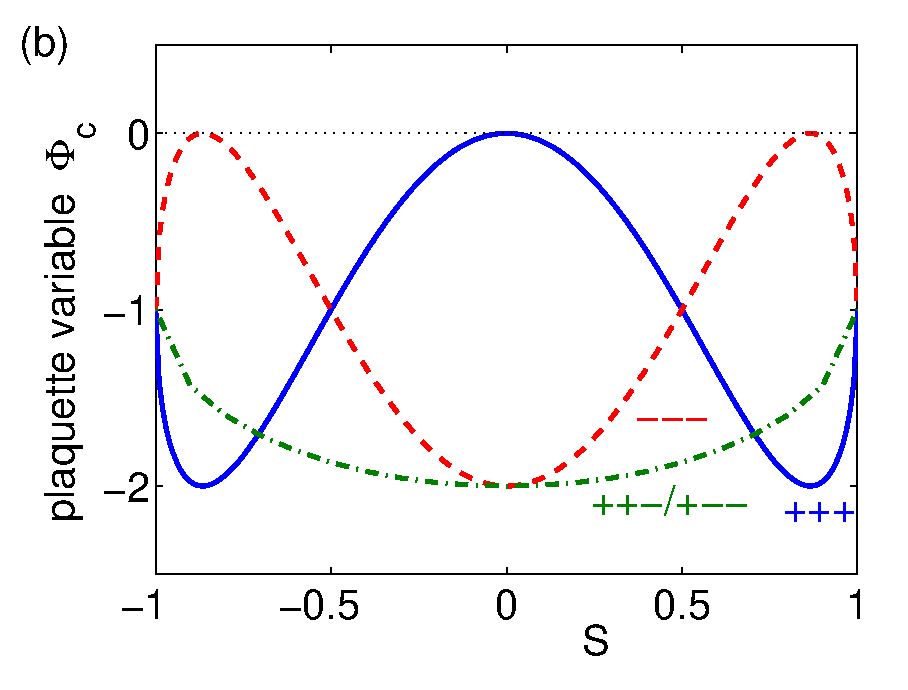
\includegraphics[width=7cm, angle=0]{pics/cycle3b_phifun}
\caption{\label{fig:cycle3}
Geometric solution of the simplest cyclic network with
3 nodes with $P_j=0$ and three links with equal
strength $K$.
(a) The black line is the solution space of the dynamical condition 
(\ref{eqn:3cycle-dc}), $S_{12} = S_{23} = S_{31} = S$
and the surface shows the relevant branches of the solution 
space of the geometrical condition (\ref{eqn:3cycle-gc}). 
One finds three intersections corresponding to three stationary states.
(b) The plaquette function \eqref{eq:phifun} along the line
$S_{12} = S_{23} = S_{31} = S$ for different branches of the
solution space. the three stationary states are characterized by 
$\Phi_c=0$. 
}
\end{figure}

Taking into account that there are two possible solutions for the
phase difference, see Eq.~(\ref{eqn:deltaS}), the geometric condition
can be written as
\bea
      \arcsin(S_{12}) + \arcsin(S_{23}) +  \arcsin(S_{31}) &=& 0    \nn \\ 
      \arcsin(S_{12}) + \arcsin(S_{23})  -  \arcsin(S_{31}) &=& \pi \nn \\ 
      \arcsin(S_{12}) - \arcsin(S_{23})  + \arcsin(S_{31}) &=& \pi \nn \\ 
   - \arcsin(S_{12}) + \arcsin(S_{23})  +  \arcsin(S_{31}) &=& \pi  
   \label{eqn:3cycle-gc} 
\eea 
Figure \ref{fig:cycle3} shows the affine set defined by 
Eq.~(\ref{eqn:3cycle-dc})  and one branch of the solution
space defined by  (\ref{eqn:3cycle-gc}). One observes that 
there are three intersections corresponding to 
three stationary states. This shows that stationary
states are generally not unique, also in the presence
of cycles.
The three remaining branches of the solution space
of Eq.~(\ref{eqn:3cycle-gc}) do not yield additional
solutions.
In the present case only one of the solutions are stable,
but this is generally not true in larger cycles as we will
show in the following.




\subsection{Frustration induces discreteness.} 
\label{eqn:sec-cycle}

We now extend the above example to a single cycle with an arbitrary number 
of nodes with the same power $P_j \equiv 0$. All links have an equal strength 
$K$ as above.
For the sake of convenience we label the nodes as $1,2,\ldots,N$ along the cycle 
and identify the node $1$ with $N+1$ and $0$ with $N$. In order to have a 
non-trivial closed cycle we need $N \ge 3$. 
The dynamic conditions for a stationary states are then given by
\bea
  && F_{j+1,j} = F_{j,j-1}  \equiv F \qquad \forall j = 1,\ldots,N  \\ 
  && |F| \le K.
\eea
For notational convenience we identify the node $1$ with $N+1$ and
$0$ with $N$. We stress that the dynamic conditions have a continuum 
of solution, i.e. all values $F$ in the interval $[-K,K]$ are allowed. 

The phase difference along the edges $(j+1,j)$ is
given by equation \eqref{eqn:deltaS}, leaving two possible solutions
$+$ and $-$. Choosing the minus sign for at least one edge $(\ell+1,\ell)$ 
yields $\widetilde K_{\ell+1,\ell}^{\rm red} = - \sqrt{K^2 - F^2} < 0$.
In this case one can show that the Hesse matrix $M$ is not positive
semi-definite such that the stationary state must be unstable. Restricting
ourselves to the dynamically stable states, we find that the phase 
differences are all equal and given by
\be
     \theta_{j+1} - \theta_j = \mbox{arcsin}(F/K).
\ee
The geometric condition now yields
\be
    N \, \mbox{arcsin}(F/K) = 0 \quad (\mbox{mod} 2 \pi),
\ee
which can be satisfied only for certain \emph{discrete} values of $F$. The
geometric condition thus induces a `quantization' of the phase differences
\be
   \theta_{j+1} - \theta_j = \frac{n}{N} 2 \pi, \qquad \mbox{with} \; 
    n = - \lfloor \frac{N-1}{4} \rfloor, - \lfloor \frac{N-1}{4} \rfloor+1, 
           \ldots, + \lfloor \frac{N-1}{4} \rfloor,
\ee
where $\lfloor \cdot \rfloor$ denotes rounding towards $- \infty$. We note that
solutions with $(\theta_{j+1} - \theta_j) = \pm \pi/2$ have stability $\mu_k = 0$
for all $k = 1,\ldots,N$. In this case dynamical stability cannot be decided by
linear stability analysis alone. For small systems it has been found that these states
are nonlinearly unstable. 
In total, we thus find $2 \times \lfloor (N-1)/4 \rfloor +1$ different stable stationary 
states.

This example is very simple but shows three important results
of ours most clearly which hold in general.
First, there can be \emph{multiple} stable equilibrium states in cyclic
networks as previously noticed by \cite{Ocha09,Tayl12,Ioni13,Meht14}. 
This fact is not fully recognized in the power engineering, probably 
because most authors in this community concentrate of fully connected 
networks which arise after a Kron reduction \cite{Tayl12,Mott13}.
Second, the oscillator model (\ref{eqn:power}) allows for 
stable equilibrium states with a persitent current around a cycle.
Interestingly, theses states are phase locked but \emph{not phase
ordered} in the sense that the phase order parameter
\cite{Stro00}
\be
   r e^{i \psi} := \frac{1}{N} \sum_j e^{i \theta_j} 
   \label{eqn:deforder}
\ee
vanishes exactly.
Third, the geometric condition induces the 
\emph{discreteness} of the phase differences
although the dynamic condition allows for continuous
values of cycle flows.


\subsection{Braess' paradox}
\label{sec:braess}

Here we introduce a special example which illustrates the
paradoxial efffects of geometric frustration most clearly.
We consider the oscillator network depicted in Fig.~\ref{fig:braess} (a)
consisting of $N=6$ nodes placed on a cyclic network.
In particular, we analyze what happens if the capacity
of the upper edge is increased from $K$ to 
$K' = K + \kappa$. 


\begin{figure}[tb]
\centering
\includegraphics[width =3.6cm, angle=0]{pics/cycleex1_a}
\includegraphics[width=4.3cm, angle=0]{pics/braess_order3}
\caption{\label{fig:braess}
Geometric frustration induces Braess' paradox.
(a) Topology of the network under consideration.
(b) Stability phase diagram: Order parameter $r$ 
as a function of $K$ and $\kappa$. No equilibrium 
state exists in the white region. 
The equilibrium can be lost when the
local transmission capacity $\kappa$ 
\emph{increases}.
}
\end{figure}

The dynamic condition for this network reads
\be
   0 = P_j + ( K_{j+1,j} S_{j+1,j}  - K_{j,j-1} S_{j,j-1} ),
   \label{eqn:dc-braess}
\ee
and $|\Delta_{j+1,j}| \le 1$, identifying node $j=7$ with $j=1$.
 For notational convenience,
we define the vector 
\be
   \vec S = (S_{6,1} ,S_{1,2}, \ldots, S_{5,6} ).
\ee
The solutions of the linear system of equations (\ref{eqn:dc-braess}) 
span a one-dimensional affine space parametrized by a real 
number $\epsilon$,
\be
   \vec S = \frac{P_0}{K} 
      \left( \vec S_a - \epsilon \, \vec S_b \right).
   \label{eqn:SaSb2}
\ee
The vector $\vec S_a = (1,1,0,-K/K',-1, 0)$ is the 
inhomogeneous solution of the linear system (\ref{eqn:dc-braess}), 
and the vector $\vec S_b = (2,1,1,2K/K',1,1)$is a homogeneous 
solution corresponding to a cycle flow.
Evaluating the condition $|S_{j+1,j}| \le 1$ yields
a necessary condition for the existstence of a stationary state
\be
     K \ge P_0.
\ee

For $\kappa = 0$ this condition is also sufficient for
the existence of a stationary state. If the capacity of the
upper link increases, $\kappa > 0$, geometric frustration
inhibits phase locking. A solution of the dynamical conditions
always  exists for   $K \ge P_0$, but this can become 
incompatible with the geometrix condtion as illustrated 
in the stability diagram  in Figure \ref{fig:braess} (b). No equilibrium
state exists in the white region of parameter space. 
In the remaining region, we have plotted the Kuramoto phase 
order parameter (\ref{eqn:deforder})
in a color color.
One clearly observes that the unstable region \emph{increases} 
with $\kappa$. This leads to the paradoxial effect that
an increase of local transmission capacity reduces
the ability of the network to support a phase locked 
equilibrium state. This behavior can also be seen as an example of 
Braess' paradox which has been first predicted for traffic 
network \cite{Brae68,12braess}.
 

\section{Multistability and the number of equilibria}

The previous examples show that there can be quite a large
number of stable equilibrium states in a cyclic network. 
In the following we derive bounds on the number of stable 
equilibria for depoending on the network structure.

\subsection{Tree network}

In the previous section we have argued that multistability
arises due to the possibility of cycle flows. In a tree there
are no cycles such that we obtain the following very strong result.

\begin{corr}
\label{eqn:corr-tree}
In a tree network, there is either no equilibrium state
or there are $2^{N-1}$ equilibrium states of which
one is stable and $2^{N-1}-1$ are unstable.
\end{corr}

\begin{proof}
By definition, a tree has $L=N-1$ edges such that the
space of solutions of the linear system (\ref{eqn:dc2a}) 
has dimension $L-N+1 = 0$. That is, there is either zero
of exactly one unique solution for the flows $F_{j,\ell}$.
In the first case no equilibrium exists. In the latter case
there are $2$ possible values for the phase difference 
for each of edge given by equation (\ref{eqn:deltaS}).
Hence there are $2^L = 2^{N-1}$ equilibrium states.
Choosing the $+$-sign in equation (\ref{eqn:deltaS}) 
yields one stable equilibrium state as shown in corrolary 
\ref{corr:stab-phasediff}.

It remains to show that all other equilibrium states are unstable.
So consider an equilibrium state with one edge with a phase difference 
that exceeds $\pi/2$. The network is a tree such that it is decomposed
into two parts which are only connected by this edge. We label the
nodes by $1,\ldots,\ell$ in one part and by $\ell+1,\ldots,N$.
in the other part. Then the Hesse matrix $M$ 
(see section \ref{sec:bifurcation})
has the form
\be
    M  = \left( \begin{array}{c|c}
    M_1 & 0     \\   \hline
    0 & M_2 \\ 
   \end{array} \right) +
    \begin{pmatrix}
       \ddots & & & & \\
       & 0 &0 & 0 & 0 &  \\
        & 0 & K^{\rm red}_{\ell,\ell +1} & -K^{\rm red}_{\ell,\ell +1} & 0 & \\
        & 0 & -K^{\rm red}_{\ell,\ell +1} & K^{\rm red}_{\ell,\ell +1} & 0 & \\
       & 0 & 0 & 0 & 0 & \\
      &  &  & & & \ddots \\
  \end{pmatrix}, 
\ee
where $K^{\rm red}_{\ell,\ell +1} < 0$
and $M_1$ and $M_2$ are defined as in equation
(\ref{eq-M}) for the two parts of the network.
Now define the vector
\be
   \vec v = ( \underbrace{1,\ldots,1}_{\ell \, {\rm times}},
                     \underbrace{0,\ldots,0}_{(N-\ell) \, {\rm times}} )^T.
\ee
Due to the structure of the matrix $M_1$ we have 
$M_1 (1,\ldots,1)^T = \vec 0$ such that
\be
   \vec v^T M \vec v =  K^{\rm red}_{\ell,\ell +1} < 0.
\ee
Thus, the Hesse matrix $A$ is not positive semi-definite, 
i.e.~it has at least one negative eigenvalue and the 
equilibrium state is unstable (cf.~lemma \ref{thm:stability-M}).
\end{proof}

\subsection{Simple cycles}
\label{sec:cycles}

For networks containing a single cycle, it is possible to derive rather
tight upper and lower bounds for the number of steady states which satisfy
$\cos(\theta_i^*  - \theta_j^*) > 0$ for all edges $(i,j)$. These states 
correspond to the normal operation of a power grid, and are guaranteed 
to be stable by corollary \ref{corr:stab-phasediff}. Other stable steady 
states can exist in particular at the border of the stable parameter 
region \cite{14bifurcation}. 
As before, we label the nodes as $1,2,\ldots,N$ along the cycle, fixing the
direction of counting in the counter-clockwise direction and identify the 
node $1$ with $N+1$ and $0$ with $N$. Likewise we fix the orientation 
of the edges $e = 1,\ldots,L$ such that $F_e>0$ describes a 
counter-clockwise flow and $F_e<0$ a clockwise flow.

We will first calculate the exact number of fixed points. However,
the result depends on one particular solution of the dynamic conditions
(\ref{eqn:dc1}), which limits its applicability. 
Therefore, we also derive lower and upper bounds for the number of 
fixed points in terms of a few simple characteristics of the grid, in 
particular the maximum partial net power. 


\begin{lemma}
\label{lem:cf-fp-corr}
Let $\vec{\phi_0}$ is a fixed point of a ring network $R$.  Then any other 
fixed point $\vec{\phi_k}$ of the same network must differ from $\vec{\phi_0}$ 
by a \emph{cycle flow} $f^{\rm cycle}(k)$.  
In other words, if $\mathbf{S}_R$ be the set 
of all fixed points of a ring network $R$, there exists a one-to-one 
function $f^{cycle}:\mathbf{S}_R\mapsto \mathbb{R}$ mapping the cycleflows to 
the set of real numbers $\mathbb{R}$.  
\end{lemma}


\begin{proof}
If $|\mathbf{S}_R|<2$  the Lemma is vacuously true.  
Suppose $\vec{\phi_0},\vec{\phi_1} \in \mathbf{S}_R$.   
Let $(F^{(0)}_1, F^{(0)}_2,\cdots,F^{(0)}_N)$ and $(F^{(1)}_1, F^{(1)}_2,\cdots,F^{(1)}_N)$ be the flows 
associated with $\vec{\phi_0}$ and $\vec{\phi_1}$.  
Using Lemma \ref{lem:flow-power}, we see that
\begin{align}
\label{}
F_{j,j+1}-F_{i-1,j}&=P_j\quad\forall j \\
F'_{j,j+1}-F'_{i-1,j}&=P_j
\end{align}
Therefore
\begin{align}
\label{}
F^{(0)}_{j,j+1}-F^{(1)}_{j,j+1}&=F^{(0)}_{j-1,j}-F^{(1)}_{j-1,j}=c,\quad\forall j\\
\Rightarrow F^{(0)}_{j,j+1}-F^{(1)}_{j,j+1}&=c,\quad\forall j.   
\end{align}
So all the flows in the second steady state differs from the first one by a 
constant amount $c$.   
Hence the function $f^{\rm cycle}(\phi_m)=F^{(m)}_{j,j+1}-F^{(0)}_{j,j+1}$ is by construction a 
one-to one function mapping each fixed point to a cycle flow.  
\end{proof}


\begin{defn}
For any ring network $R$ and a fixed point $\vec{\phi}$, the \emph{winding 
number of the fixed point} is defined as 
\begin{align}
\label{def:wnum}
\omega(\vec{\phi})&=\frac{1}{2\pi}\sum_{\text{all edges }e} \arcsin{\frac{F_e}{K_e}}\\
&=\frac{1}{2\pi}\sum_{\text{all edges }e} \arcsin{\frac{F_e^{(0)}+f^{\rm cycle}}{K_e}}
\end{align}
\end{defn}



\begin{lemma}
\label{lemma-cycle}
For a ring network $\R_N$, the number of equilibrium state which satisfies 
$\cos(\theta_i^*  - \theta_j^*) > 0$ for all edges $(i,j)$  (denoted by $\N$)
is given by 
\begin{align}   
   \N =  \floor{\frac{1}{2\pi} \sum_j\arcsin\left(\frac{F_{j+1,j}^{(0)}+f^{\rm cycle}_{\rm max}}{K_{j+1,j}}\right) }
    - \floor{\frac{1}{2\pi}\sum_j\arcsin\left(\frac{F_{j+1,j}^{(0)}+f^{\rm cycle}_{\rm min}}{K_{j+1,j}}\right) }
\end{align}
where $\floor{\cdot}$ denotes rounding towards $-\infty$.
$F_{ij}^{(0)}$ is one particular solution to the dynamic condition (\ref{eqn:dc1})
and
\begin{align}
   \label{eqn:def-Fmaxmin}
   f^{\rm cycle}_{\rm max} &= \min_j \left( K _{j+1,j} - F_{j+1,j}^{(0)} \right), \nn \\
   f^{\rm cycle}_{\rm min} &= \max_j  \left( - K _{j+1,j} - F_{j+1,j}^{(0)} \right).
\end{align}
\end{lemma}

\begin{proof}
Suppose we have one steady state $\vec{\phi_0}$
with the flows $F_{ij}^{(0)}$ and analyze (as per Lemma \ref{lem:cf-fp-corr})
which cycleflow values $f^{\rm cycle}$ lead to different valid steady states. 
First, the value of the cycle flows is bounded both above and below
since the flow $F_{j,j+1}$ along each edge cannot exceed in 
absolute value the capacity $K_{j,j+1}$:
\begin{align}
  \label{eq:fp_limits}
  f^{\rm cycle}_{\min} & \leq f^{\rm cycle} \leq f^{\rm cycle}_{max}\\
  f^{\rm cycle}_{\max}&=\min_{j} \left(K_{j,j+1}-F^{(0)}_{j,j+1} \right)\\
  f^{\rm cycle}_{\min}&=\max_{j} \left(-K_{j,j+1}+F^{(0)}_{j,j+1} \right)\\
\end{align}

Second, all steady state have to satisfy the geometric condition (\ref{eqn:deltaS})  . 
Here we have to take into account only the $+$-sign as we consider only states in 
normal operation, i.e.~states with $\cos(\theta_i - \theta_j) > 0$ for every
edge $(i,j)$. The geometric condition thus reads
\be
    \omega(f^{\rm cycle}) \in \mathbb{Z},
\ee
where the winding number is given by
\be
   \omega(f^{\rm cycle}) = \frac{1}{2\pi} \sum_j\arcsin\left(\frac{F_{j+1,j}^{(0)}+f_c}{K_{j+1,j}}\right).
\ee
Using the bound for the cycle flow strength (\ref{eq:fp_limits}), we find that the winding 
number is also bounded
\begin{align}
   \omega(f^{\rm cycle}_{\min}) \le \omega \le \omega(f^{\rm cycle}_{\max})
  \label{eq:lim-omega}
\end{align}
such that the distinct fixed points correspond to the following values of the winding number. 
\be
    \omega_{\rm fixed point} = \floor{ \omega(f^{\rm cycle}_{\min}) } + 1,
           \floor{ \omega(f^{\rm cycle}_{\min})  } + 2, \ldots,
           \floor{ \omega(f^{\rm cycle}_{\max})  } ,
\ee
Counting these values and inserting the values for $f^{\rm cycle}_{\min}$
and $f^{\rm cycle}_{\max}$ then yields the the number of fixed points $\N$.
\end{proof}


For practical applications is its desirable to determine the number of steady states
from the properties of the network alone, without referring to a particular solution
$F^{(0)}$. To obtain suitable bounds for the number of steady states $\N$, we 
first define some properties which characterize the network.

\begin{defn} 
For a ring network $\R_N$ with $N\in \mathbb{N}$ nodes indexed by $1,2,\cdots,N$
along the cycle, a \textbf{fragment} $\F_{i,j}$ is defined as the path starting at node $i$ 
and ending at node $j$. For any fragment $\F_{i,j}$, the \textbf{partial net power} 
$\bar{P}_{ij}$ is defined as
\be
   \bar{P}_{ij}=\sum_{k=i}^j P_k.  
\ee
and the \textbf{maximal partial net power} is defined as
\begin{align}
  \label{def:mpnp}
   \bar{P}_{\max}=\max_{i,j} \bar{P}_{i,j}.
\end{align}
This concept is illustrated in Fig.~\ref{fig:pmax}
Furthermore we define the maximum and minimum transmission capacities
\be
    K_{\rm max} = \max_{j} K _{j+1,j} 
     \quad \text{and} \quad
    K_{\rm min} = \min_{j} K _{j+1,j}.
\ee
\end{defn}

\begin{figure}[!htp]
\begin{center}
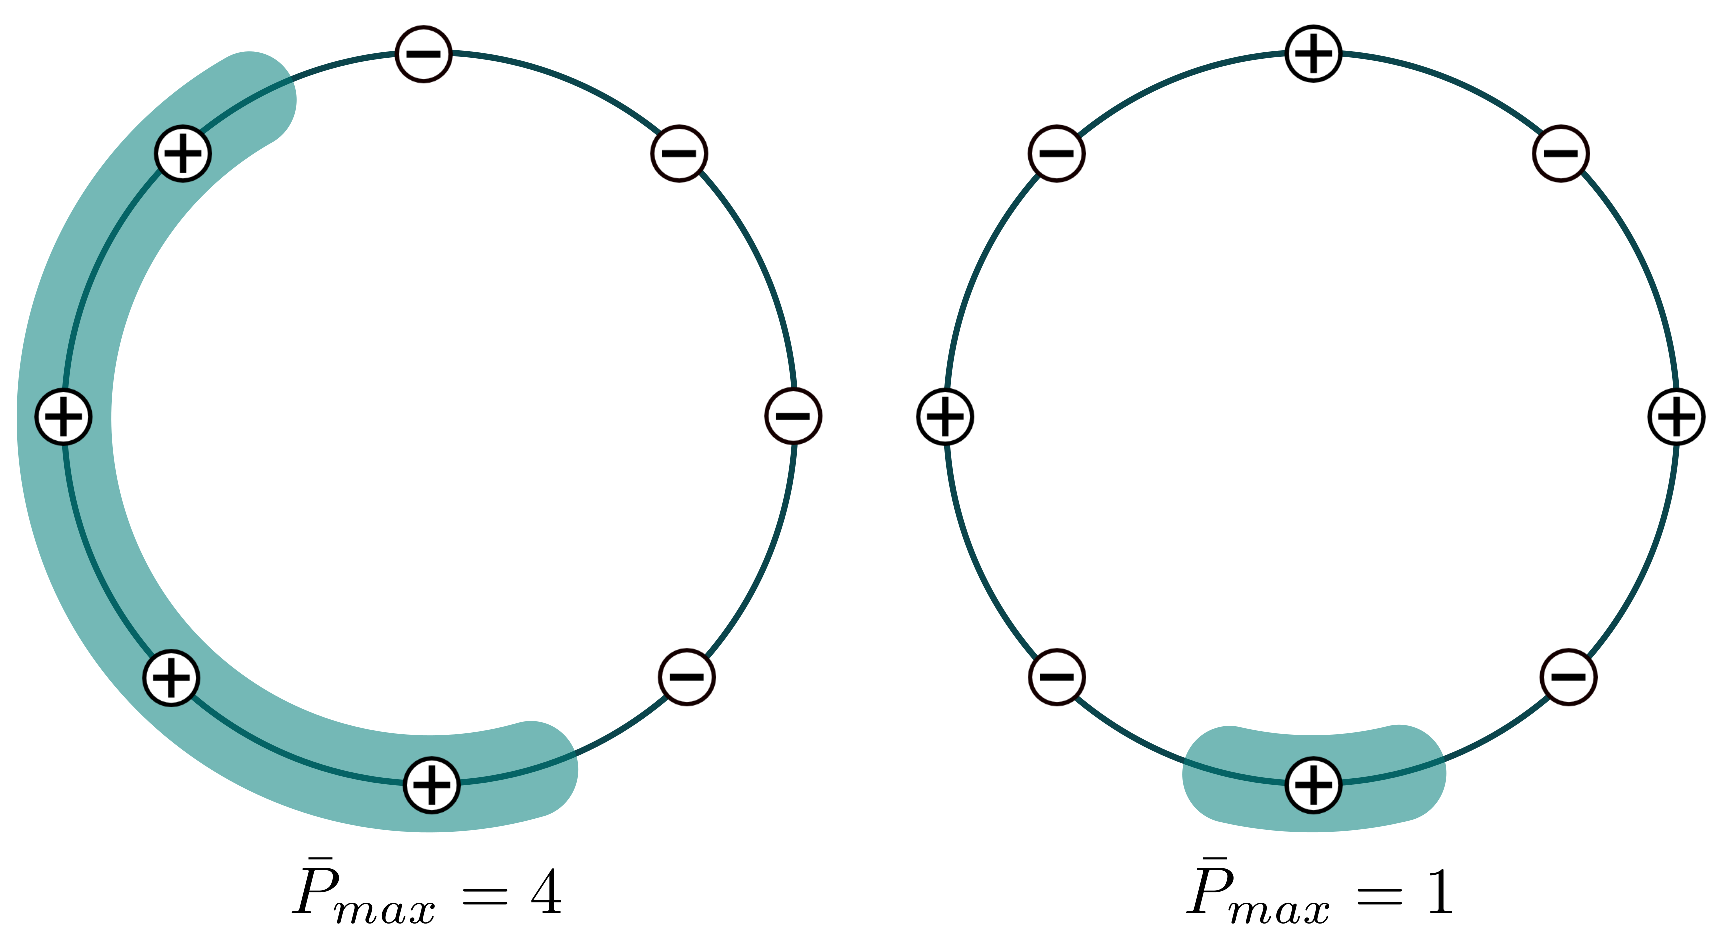
\includegraphics[width=0.6\columnwidth]{pics/pmax_compare}
\end{center}
\caption{
\label{fig:pmax}
  The maximum partial net power $\bar{P}_{\max}$ in different ring networks.
}
\end{figure}

\begin{lemma}
\label{lem:flow-power}
For any ring fragment $\F_{i,j}$, the partial net power is equal to the net outwards flow:
\begin{align}
  \label{eq:glow-power}
  \bar{P}_{ij}=F_{j+1,j}-F_{i-1,i}
\end{align}
and
\begin{align}
   \bar{P}_{\max} = \max_j F_{j+1,j} - \min_{i} F_{i-1,i} \, .
\end{align} 
\end{lemma}


\begin{corr}
\label{corr:hom-ring}
For a ring network $\R_N$, the number of equilibrium state which satisfies 
$\cos(\theta_i^*  - \theta_j^*) > 0$ for all edges $(i,j)$  (denoted by $\N$)
is bounded from above and below by
\begin{align}
   0  \leq \N \leq 2 \times \floor{ \frac{N-1}{4} }  +1 
\end{align}
and by
\begin{align}
   \N & \geq \floor{ \frac{N}{2\pi} 
           \frac{2 K_{\rm min} - \bar P_{\rm max}}{K_{\rm max}} } \nn \\
   \N & \leq \floor{ \frac{N}{4} + \frac{N}{2\pi}
          \arcsin \left(  \frac{2 K_{\rm max} - \bar P_{\rm max}}{K_{\rm min}} -1  \right) }+1.
     \label{eqn:bounds:homring2}      
\end{align}
\end{corr}

\begin{proof}
According to lemma \ref{lemma-cycle} the number of steady states $\N$ 
is given by
\begin{align}
    \N = \floor{\omega(f^{\rm cycle}_{\max})} -
       \floor{\omega(f^{\rm cycle}_{\min})} \, .
\end{align}  
We make use of the fact that the arcsin function is bounded, 
$\arcsin(\theta_{j+1}-\theta_j) \in (-\pi/2,+\pi/2)$, such that   
\begin{align}
   2\pi \omega(f^{\rm cycle}_{\rm max}) &= 
       \sum_j \arcsin \left(\frac{F_{j+1,j}^{(0)}+F'_{\rm max}}{K_{j+1,j}}\right)
     < N \frac{\pi}{2}   \nn \\
    2\pi \omega (f^{\rm cycle}_{\rm min}) &= 
       \sum_j \arcsin \left(\frac{F_{j+1,j}^{(0)}+F'_{\rm max}}{K_{j+1,j}}\right)
     > - N \frac{\pi}{2}    
\end{align}
This proves the first part of the corollary.

To proof the second part, we start from 
\begin{align}
   \label{eq:nf-bounds}
   \floor{\omega(f^{\rm cycle}_{\rm max}) - \omega(f^{\rm cycle}_{\rm min})} 
      &\leq \N \leq 
    \floor{\omega(f^{\rm cycle}_{\rm max}) - \omega(f^{\rm cycle}_{\rm min})} +1  
\end{align}
Now one can obtain upper and lower bounds for all terms in the
sum using the trigonometric relation 
\begin{align}
   \label{eqn:xy-arcsin}
   x-y\leq \arcsin(x)-\arcsin(y)\leq \frac{\pi}{2}x-y
\end{align}
which holds for all $-1\leq y \leq x \leq 1$.

\debsankha{(This was a mistake: for all $-\frac{\pi}{2}\leq y \leq x \leq \frac{\pi}{2}$.)}

\begin{minipage}{\columnwidth}
\debsankha{@Dirk: I had been using the other upper bound 
$x-y\leq \arcsin(x)-\arcsin(y)\leq \frac{\pi}{2}(1-(x-y))$ you suggested in 
the latest revision.  I think your suggestion is just as tight as the old one, 
plus much cleaner, 
Therefore I am changing this section.  }
\includegraphics[width=0.6\columnwidth]{pics/arcsin_upper_bounds}
\end{minipage}



This yields 
\begin{align}
\label{eq:q-bounds}
   \frac{1}{2\pi} \sum_j\frac{\Delta f^{\rm cycle}}{K_{j+1,j}} &\leq 
    \omega(f^{\rm cycle}_{\rm max}) - \omega(f^{\rm cycle}_{\rm min}) \leq 
    \frac{N \pi}{4} +  \frac{1}{2\pi} \sum_{j} \arcsin\left(\frac{\Delta f^{\rm cycle}}{K_{j+1,j}} - 1\right),
\end{align}
where we define $\Delta f^{\rm cycle} = f^{\rm cycle}_{\rm max}) - f^{\rm cycle}_{\rm min})$.
Furthermore, this quantity can be bounded as
\begin{align}
  \Delta f^{\rm cycle} &= \min_j \left( K _{j+1,j} - F_{j+1,j}^{(0)} \right) -
                     \max_j  \left( - K _{j+1,j} - F_{j+1,j}^{(0)} \right) \nn \\
               & \geq 2 K_{\rm min} +  \min_j \left( - F_{j+1,j}^{(0)} \right)
                      - \max_j  \left( - F_{j+1,j}^{(0)} \right) \nn \\
               & = 2 K_{\rm min} +  \max_j \left( F_{j,j+1}^{(0)} \right)
                      - \max_j  \left( - F_{j+1,j}^{(0)} \right) \nn \\       
               & = 2 K_{\rm min}- \bar P_{\rm max}  
\end{align}
such that the fraction in equation (\ref{eq:q-bounds}) becomes
\begin{align}
     \frac{\Delta f^{\rm cycle}}{K_{j+1,j}} \geq  \frac{2 K_{\rm min}- \bar P_{\rm max}}{K_{\rm max}} .
\end{align}
In a similar way we find $\Delta f^{\rm cycle} \leq 2 K_{\rm max}- \bar P_{\rm max}$ such that
\begin{align}
   \arcsin\left(\frac{\Delta f^{\rm cycle}}{K_{j+1,j}} - 1 \right) \leq
      \arcsin\left(\frac{2 K_{\rm max}- \bar P_{\rm max}}{K_{\rm min}} - 1 \right) .
\end{align}
Substituting these bounds into equation (\ref{eq:q-bounds}) yields
\begin{align}
  \omega(f^{\rm cycle}_{\rm max}) - \omega(f^{\rm cycle}_{\rm min})
      & \geq \frac{N}{2\pi} \, \frac{2 K_{\rm min}- \bar P_{\rm max}}{K_{\rm max}} \nn \\
  \omega(f^{\rm cycle}_{\rm max}) - \omega(f^{\rm cycle}_{\rm min})
       & \leq \frac{N \pi}{4} + 
      \frac{N}{2\pi}  \arcsin\left(\frac{2 K_{\rm max}- \bar P_{\rm max}}{K_{\rm min}} - 1 \right) 
\end{align}
which completes the proof.
\end{proof}



\begin{corr}
\label{cor:high-k-nf}
\label{corr:nomult-3}
For homogeneous rings $\R_N$, i.e.~$K_{i,i+1}=K$, equation (\ref{eqn:bounds:homring2})      
simplifies to
\begin{align}
   \frac{N}{\pi}-\frac{N\bar{P}_{\max}}{2K\pi} \leq \N \leq \frac{N}{2} - \frac{N\bar{P}_{\max}}{4K}+1.
\end{align} 
Ring networks $\R_N$ with $N \le 4$ don't have multiple stable fixed points.
A homogeneous ring network $\R_{N}$ with $N \ge 7$ nodes 
will have multiple stable fixed points $(\N \ge 2)$ if 
\begin{align}
   \label{crit:mult-fp}
   \bar{P}_{\max} \le 2 K_{\rm min} - \frac{4 \pi }{N} K_{\rm max} \, .
\end{align}
\end{corr}
These relations can be proven by simply evaluating the bounds in corollary  
\ref{corr:hom-ring}.

\dirk{XXX Note to Debsankha: The last relation holds only if the denominator is
positive which is the case for $N \ge 2\pi$. Please check factors of $2$, I obtained
a difference to your result. How can we proof that there is no steady state for $N=3$? I am 
sure that this is correct, but I don't see it directly. XXX}

\begin{figure}[htb]
\label{fig:scaling-nf}
\begin{center}
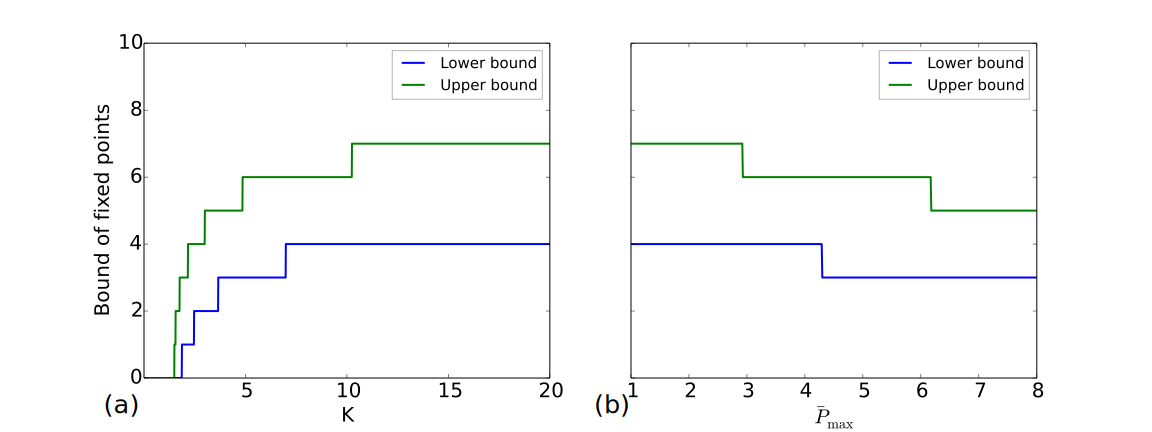
\includegraphics[width=\columnwidth]{pics/num_fps_k_p_ring}
\caption{
Upper and lower bounds for the number of steady states $N_f$ 
for a sample 16 element ring as a function of (a) $K$, which is same for all 
edges, while $\bar{P}_{\max}=3$, and (b) $\bar{P}_{\max}$ while $K=10$.  }
\end{center}
\end{figure}

We illustrate how the bounds scale with the connectivity $K$  and $\bar{P}_{\max}$ for a sample ring 
of size $16$ in  Fig \ref{fig:scaling-nf}. We see in Fig \ref{fig:scaling-nf} 
(a) that increasing $K$ results in more stable fixed points.  Whereas Fig 
\ref{fig:scaling-nf} (b)  demonstrates that if the power generators 
$(P_j\ge  0)$ are clustered together, then the system has less fixed points, 
as opposed to the case where they are more distributed.   

\dirk{XXX This old old remark of mine is obsolete with the new figure, is it?
We should discuss the role of $\bar P_{\rm max}$ in more detail. Actually it says:
The more distributed the generators are in the grid ($\bar P_{\rm max}$ small), the more steady 
states exist. We even have an expression for the critical coupling in terms of the maximum
partial net power! This should be stated in an own corollary, otherwise this cool result might 
be overlooked. But we have to discuss the meaning of $\bar P_{\rm max}$ in more detail
to reveal its physical importance. A figure would be nice. XXX}


\dirk{XXX I revised the paper up to this point. Dirk, 22/5/15 XXX}

\dirk{XXX Let's get rid of this section. Either include reusaltsd above or throw them out
completely. XXX}


\subsection{More corrolaries}
\begin{lemma}
\label{}
Number of fixed points scales with the average length of cycles.  
\end{lemma}

\dirk{XXX To include this result we have to make it more precise. XXX}

\begin{corr}
\label{cor:high-k-nf}
A homogeneous ring network $R_{N}$ with $N$ nodes 
 will have multiple stable fixed 
points if 
\begin{align}
\label{crit:mult-fp}
K\geq \frac{\bar{P}_{\max}}{2\left(1-\frac{\pi}{N}\right)}
\end{align}
\end{corr}

\dirk{XXX I merged these results into corollary 4, but I have a different factor on 2. Please check. XXX}

\begin{corr}
\label{corr:nomult-3}
A homogeneous ring network of sixe $N$ doesn't have multiple fixed point for 
$N\leq 3$.  
\end{corr}

\dirk{XXX I merged these results into corollary 4. IThere are no multiple fixed points for $N=4$, 
but this is not yet included in the proof. XXX}


\begin{corr}
As $K$ is decreased, the fixed points with higher \emph{winding number} 
\eqref{eqn:gc2} will vanish. From another point of view, the fixed points with 
largest infinity norm
\[
\max_j\left|F_{j,j+1}\right|
\]
will be the first ones to vanish.  
\end{corr} 

\dirk{XXX This corollary is nice, we can put it into the text directly after corollay 4 
without any more need for discussion. XXX}

\begin{lemma}
In a Kuramoto network, critical coupling scales as:
\[
K_c\propto \frac{\sum P_j}{N_E}
\]

\dirk{XXX To include this result we have to make it more precise. XXX}

Numerics approaches: \\
a. Devise an algorithm to calculate the RHS.   \\
b. Generate graphs suitably so that RHS is trivial to compute.  
\end{lemma}



\subsection{Inconsistencies in the literature}

\dirk{XXX Discussion: Similar results by [Ochab+Gora]. Compare!
The two corollaries above contradict [Barahova et al.]. Please include correct references. XXX}

\debsankha{TODO: Barahona et al claimed things that are not true.}  



\subsection{Complex networks}

\begin{defn}
For a connected  graph $G(V,E)$, we define a \emph{simple cycle set} $F$ as an 
ordered set containing the basis cycles of $G$
\[
F=\left[C_1, C_2,\cdots, C_{\gamma} \right],
\]
where 
\[
C_l=\left[v_{l1},v_{l2},\cdots, v_{ln}\right]
\]
%Without loss of generality, we order the nodes in a cycle $C_l$ in 
%counter-clockwise manner.   


It can be shown that 
$|F|=\gamma=|E|-|V|+1$ (cf. \debsankha{add ref}).  
\end{defn}


\begin{lemma}
\label{lem:cf-fp-corr-planar}
Let $\mathbf{S}_G$ be the set of all fixed points of a network $G$ 
satisfying the normal operation criteria \eqref{def:normalop}.
Then there exists a one-to-one function $\vec{f_c}:\mathbf{S}_R\mapsto \mathbf{R}^{\gamma}$ 
that maps each fixed point to a \emph{cycle flow vector}.  

\end{lemma}
\begin{proof}
Using the identical reasoning used in Lemma \ref{lem:cf-fp-corr} to arbitrary 
graphs instead of simple cycle, the proof follows.  
\end{proof}


\subsubsection{Planar graphs}
For planar graphs one can generalize the results of the section \ref{sec:cycles} in 
a straightforward way. To this end we define certain relevant quantities.  

\begin{defn}
\label{def:wvec}
For a connected planar graph $G$, and a certain distribution of generators $\vec{P}$, let $\vec{\phi^*}\in \mathbb{R}^{|V|}$ be a 
steady state.  Then the \emph{winding vector} $\vec{\omega}(\vec{\phi^*})$ is defined as:

\begin{align*}
\omega_l &= \frac{1}{2\pi} \sum_{e\in C_l} \arcsin{\frac{F_e}{K_e}}, \quad \forall 1 \leq l 
\leq \gamma\\
&=\frac{1}{2\pi} \sum_{e\in C_l} \arcsin{\frac{F_e^0+f^{cycle}_l-f^{cycle}_{n(e)}}{K_e}}
\end{align*}
\end{defn}

Here we have used the notation that for every edge $e\in C_l$, $n(e)$ is the 
index of the cycle adjacent to $C_l$ sharing edge $e$.  


\begin{lemma}
\label{lem:wind-fp-corr-planar}
For a planar network, if $\vec{\omega}(\vec{\phi_1})=\vec{\omega}(\vec{\phi_2})$ and both 
$\vec{\phi_1}$ and $\vec{\phi_2}$ satisfy \eqref{def:normalop} then 
\begin{align}
\label{}
\vec{\phi_1}&=\vec{\phi_2}. 
\end{align}
\end{lemma}

\begin{proof}
Suppose to the contrary.   

Let $\vec{f}$ and $\vec{f'}$ be the two cycleflow vectors as defined in 
\ref{lem:cf-fp-corr-planar} for $\vec{\phi_1}$ and $\vec{\phi_2}$ 
respectively.   

%Then, by virtue of our assumption 


Now consider the difference in cycleflows in each cycle between the two fixed points
\[
\{f'_l-f_l:1\leq l \leq \gamma\}
\]

Let $C_k$ be the cycle for which this quantity is largest

\begin{align}
\label{}
f'_k-f_k & \geq f'_l-f_l,\quad \forall l\neq k.  
\end{align}

Then we have

\begin{align}
\label{}
f'_k-f'_{n(e)} & \geq f_k-f_{n(e)} \quad\forall e\in C_k\\
\sum_{e\in C_k} \arcsin{\frac{F_e^0+f'_k-f'_{n(e)}}{K_e}} &\geq \sum_{e\in C_l} \arcsin{\frac{F_e^0+f_k-f_{n(e)}}{K_e}}\\
\Rightarrow \vec\omega_l(\vec{\phi_1})&\neq 
\vec\omega_l(\vec{\phi_2})\quad\text{ (using Definition \ref{def:wvec})}
\end{align}

This contradicts our contrary assumption.   
This concludes the proof.  
\end{proof}
 


\begin{lemma}
\label{}
Let $G$ be a planar network with simple cycle set $F=[C_1,C_2,\cdots,C_{\gamma}]$. Let $l_b$ be the length of the \emph{boundary} 
of $G$, i.e. the number of edges that are part of only one cycle.  Let 
$\omega^{\max}_l$ and $\omega^{\min}_l$ be the maximum and minimum winding 
number respectively for each cycle $C_l\in F$, as determined by \eqref{eq:lim-omega}.

Then the number of fixed points of a planar network is given by the total number of 
integer solutions to the linear inequality
\begin{align}
\label{}
-\frac{l_b}{4} \leq \sum_{l=1}^{\gamma} \omega_l \leq \frac{l_b}{4},
\end{align}
subject to the constraints
\begin{align}
\label{}
\omega^{\min}_l \leq \omega_l \leq \omega^{\max}_l.  
\end{align}
\end{lemma}



\subsubsection{Complete graph}
\begin{theorem}
\label{}
A completely connected network $G(n)$ has only one fixed point satisfying 
\eqref{def:normalop}. 
\end{theorem}

\begin{proof}
Since $G(n)$ is completely connected, we can choose simple cycle set $F$ of to 
consist of triangles, for example:
\[
F=[(n_1, n_2, n_3), (n_2,n_3,n_4),\cdots, ].
\]

Suppose $\vec{\phi^*}$ is a fixed point of a completely connected network.   
From Lemma \ref{lem:cf-fp-corr-planar}, we see that any other fixed point, if 
it exists, must consist of cycleflows in the triangles that make up $F$.   
Now, in order to satisfy \eqref{def:normalop}, the new cycleflows must cause the 
phase difference along the cycle to change by a multiple of $2\pi$.  

However, since phase difference along an edge can be maximally $\frac{\pi}{2}$ 
as per our constraint \eqref{def:normalop}, the phase difference in the whole 
cycle can change by at most $\frac{3\pi}{2}$.   

Therefore another fixed point cannot exist in a completely connected network.  
\end{proof}


\section{Old stuff}

\subsection{Fully connected graph}

\dirk{XXX Put in our theorem. XXX}

\dirk{XXX Compare results to [Taylor]: Only one fixed point if network is very dense. XXX}

\begin{lemma}
In a Kuramoto network, critical coupling scales as:
\[
K_c\propto \frac{\sum P_j}{N_E}
\]

Numerics approaches: \\
a. Devise an algorithm to calculate the RHS.   \\
b. Generate graphs suitably so that RHS is trivial to compute.  
\end{lemma}
\debsankha{cite Peter Menck's dead end paper}

\subsection{Planar graphs}

For planar graphs one generalize the results of the section \ref{sec:cycles} in 
a straightforward way. In particular, an upper bound for the number of stationary states
in normal operation is simply obtained by multiplying the upper bound for the 
elementary cycles of the network. To prove this statement we first have to establish
a rather technical result.

\dirk{XXX Put in our lemma and theorem. XXX}

\subsection{Old stuff}

\dirk{XXX To be deleted. XXX}

\begin{corr}
The number of equilibrium state which satisfies 
$|\theta_i^*  - \theta_j^*| \le \pi/2$ for all edges $(i,j)$
is bounded by
\be
   \prod_{c \in \rm{fundamental \, cycle}} \left\lfloor \frac{N_c}{2} \right \rfloor,
   \label{eqn:numsol-cycle}
\ee
where $N_c$ is the number of nodes of the cycle $c$ and
the product is taken over the $L-N+1$ fundamental cycles
of the network. For $L = N-1$ (no cycles) the number of 
solutions is bounded by $1$.

\debsankha{Now obsolete.}
\end{corr}

\begin{proof}
Consider first a network with a single cycle of the network and a given 
equilibrium state. All other solutions of the dynamical condition (\ref{eqn:dc1}) 
can be obtained by adding a cycle flow $F'$. Furthermore, the equilibrium
states have to satisfy the geometric condition  
 \be
    \Delta \Phi(F') = 2 \pi m, \qquad m \in \mathbb{Z},
   \label{eqn:gc-proof}
\ee
where the phase change along the cycle is given by
\be
   \Delta \Phi(F') := \sum_{(i,j) \in {\rm cycle}} \arcsin
    \left( ( F^{(0)}_{ij} + F') /K_{ij} \right).  
  \label{eqn:phase-proof}
\ee
Here we can use the fact that $|\theta_i^*  - \theta_j^*| \le \pi/2$ 
holds by assumption for all edges $(i,j)$ such that only the plus 
sign in equation (\ref{eqn:deltaS} ) has to be considered. 

We note that the arcsin is strictly monotonous on the interval 
$(-1,+1)$. Thus, also the phase difference along the cycle as
a function of the cycle flow (\ref{eqn:phase-proof}).
is monotonous. Furthermore the arcsin is bounded such that
\be
   \Delta \Phi(F') \in N_c [-\pi/2, \pi/2].
    \label{eqn:bound-proof}
\ee
All equilibria must satisfy the geometric condition (\ref{eqn:gc-proof}).
The function $\Delta \Phi(F')$ is monotonic, such that each value 
of $m$ gives rise to at most one solution for the cycle flow $F'$. 
As the value $ \Delta \Phi(F')$ is bounded by \ref{eqn:bound-proof}, 
the total number of solutions is also bounded by $\lfloor N_c/2 \rfloor$,
where $\lfloor \cdot \rfloor$ denotes rounding towards $-\infty$.
 
In a complex network we have $L-N+1$ linearly independent
cycle flows, one for each of the fundamental cycles of the
network. For each of the fundamental cycles the number
of allowed values of the cycle flow is bounded by 
$\lfloor N_c/2 \rfloor$, 
where $N_c$ is the number of nodes in the respective cycle. 
Therefore the total number of equilibrium states is given by 
the product of these numbers
\be
   \prod_{c \in \rm{fundamental \, cycle}} \left\lfloor \frac{N_c}{2} \right \rfloor.
\ee

\debsankha{(\textbf{XXX: Problem:} Can we really multiply the number of cycle flow of each cycle? 
What if they are dependent? What if corresponding to one value of $\Delta\Phi$, 
there are multiple cycle flow combination: $F_1',F_2',\cdots$?)}
If there is no cycle ($L=N-1$), we have a tree network for which
the number of equilibrium states is given in corrolary 
\ref{eqn:corr-tree}.
\end{proof}

We note that the cycle decomposition of a network is generally not 
unique, while the number of fundamental cycles is given by $L-N+1$.
In order to obtain a bound for the number of solutions it is
thus most zweckmaessig to pick a decomposition which minimizes
the product (\ref{eqn:numsol-cycle}). We further note that the bound is tight. 
In fact the number of equilibrium states attains the bound for the example 
discussed  in section \ref{eqn:sec-cycle} attains this bound. However, one has to 
keep in mind that not all stable equilibrium states are of the form
discussed in this corollary [Manik, 2014].

\begin{corr}
In a fully conencted network there is at most one equilibrium state which
satisfies $|\theta_i^*  - \theta_j^*| \le \pi/2$ for all edges $(i,j)$.
\debsankha{merge with Corr \ref{corr:nomult-3}}
\end{corr}

\begin{proof}
In a fully connected network the cycle space is spanned by all triangles.
For a triangle we have $\lfloor N_c/2 \rfloor = \lfloor 3/2 \rfloor = 1$ 
such that the number of solutions of the given kind is one.
\end{proof}


\section{Conclusion}



\dirk{XXX Marc XXX}




% --- Literatur -------------------------------------------------------------------

\bibliography{frustration}
\bibliographystyle{apsrev}


\end{document}
